\section{Risk Management}
\label{sec:risk}
\lhead{\thesection \space Risk Management}

\subsection{Plan Risk Management}
This chapter will describe the project related risks and the impact of these risks to the project. Risk management is a continuous process where risks have to be evaluated continuously with all stakeholders to ensure a proper risk assessment. To execute a proper risk management, there are 5 important steps that needs to be executed.
\newline
\newline
Step 1: Identify the Risk.\newline
Step 2: Analyze the risk.\newline
Step 3: Evaluate or Rank the Risk.\newline
Step 4: Treat the Risk.\newline
Step 5: Monitor and Review the risk.\newline
\newline
Together these 5 risk management process steps combine to deliver a simple and effective risk management process.
In this project only the most relevant risk criteria are assessed even though there are many more risks that could be evaluated.

\subsection{Identify Risks}
Is the process of determining which risks may affect the project and documenting their characteristics.
As part of the Sofa project the assessment of risks for the three epics in conjunction with our customer.
Continuously analyzing and evaluating risks is an important task of project management. Even in early stages of the project evaluated risks can be tackled and occurrence of likelihood minimized.
In this connected.Football 3 risk breakdown structures are created.
One for every epic. 3 levels of risks are determined, where level one is the epic, level two the involved party and level three the occurring issue. All risks are evaluated against the seriousness and likelihood of occurrence.

\begin{table}[!ht]
  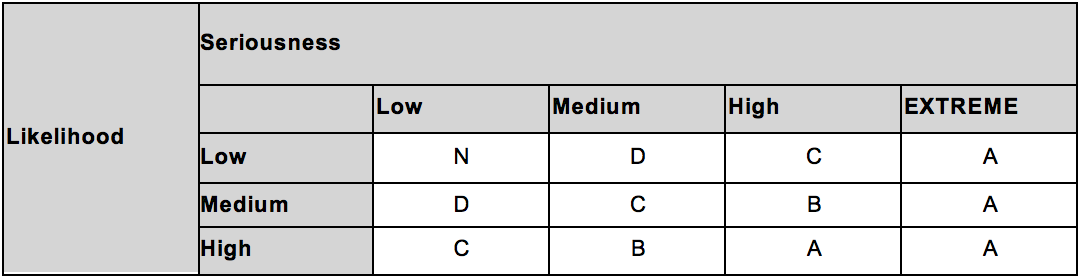
\includegraphics[width=\linewidth]{content/diagram/risk/risk_grading.png}
  \caption{Risk matrix}
\end{table}
\newpage

\subsubsection{Epic 1}
In the epic "Vote4Fun" the most influential risk is that the group of students is not able to learn the necessary knowledge to integrate the epic of the customer. 
\newline
To ensure that missing knowledge is learned within appropriate time students need to spend time on their own to compensate that knowledge and reduce the likelihood of that risk.

\begin{table}[!ht]
  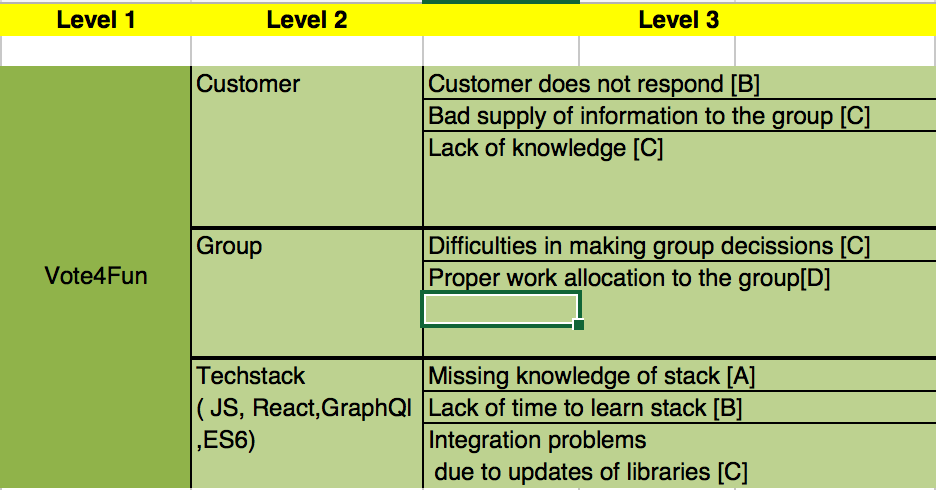
\includegraphics[width=\linewidth]{content/diagram/risk//vote4fun.png}
  \caption{Epic one}
\end{table}
\newpage
\subsubsection{Epic 2}
In the epic "Promotion Code" the most influential risk is the lack of knowledge on how to solve and implement the promotion code for certain users to enter the app. 
\newline
To reduce the likelihood of the customer who does not respond students shall deliver quality to the customer to keep him satisfied over the project life cycle.
\begin{table}[!ht]
  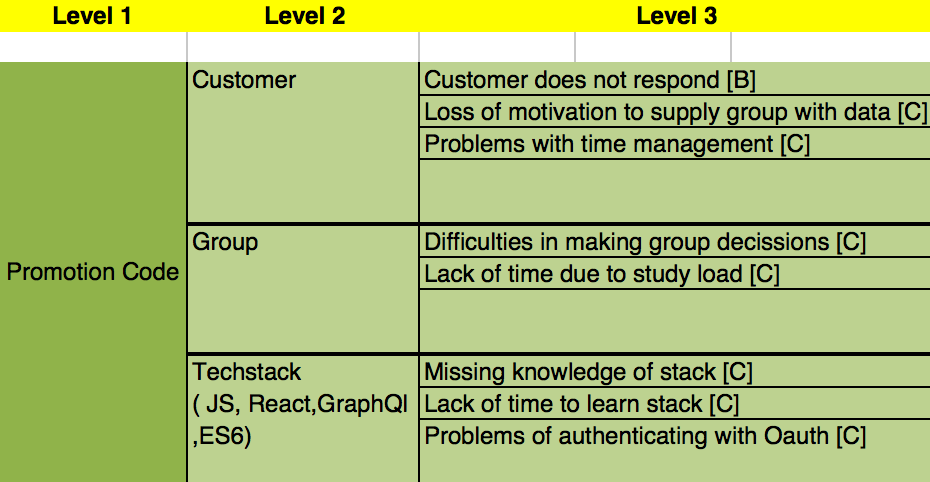
\includegraphics[width=\linewidth]{content/diagram/risk/promotioncode.png}
  \caption{Epic two}
\end{table}

\newpage
\subsubsection{Epic 3}
In the epic "group extension" the most influential risk is that we run out of time due to the workload of the first two epics.
\newline
To minimize the likelihood of occurrence that students will encounter problems due to the lack of time students need to have a structured set up of their sprint planning to always have an overview of their current project status.
\begin{table}[!ht]
  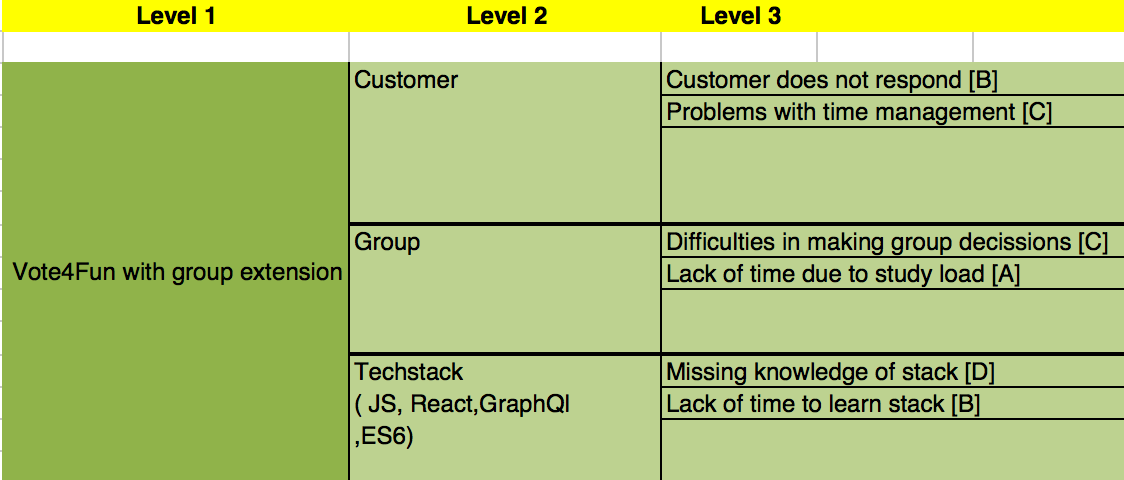
\includegraphics[width=\linewidth]{content/diagram/risk/groupextension.png}
  \caption{Epic three}
\end{table}

\subsection{Identification}
The objective of risk identification is the early and continuous identification of potential risks that can affect the project delivery. It is crucial for efficient risk management. If the risk occurs it will have negative (or sometimes positive) impact on the project's ability to achieve performance or capability outcome goals. Through the whole project life cycle this is an continuously iterative process that needs to be repeated. In the previous chapter the risks got analyzed and selected. 




